\documentclass[aspectratio=169,12pt]{beamer}
\usepackage[utf8]{inputenc}
\usepackage{amsmath, amssymb}
\usepackage{booktabs}
\usepackage{colortbl}
\usepackage{hyperref}
\usepackage{listings}
\usepackage{tikz}
\usetikzlibrary{arrows.meta, positioning, shapes.geometric, calc}
\usetheme{Madrid}

% Define colors for registers
\definecolor{r1color}{RGB}{255,0,0}
\definecolor{r2color}{RGB}{0,128,0}
\definecolor{r3color}{RGB}{255,165,0}
\definecolor{r4color}{RGB}{128,0,128}
\definecolor{r5color}{RGB}{0,0,255}
\definecolor{r6color}{RGB}{255,165,0}
\definecolor{r7color}{RGB}{0,0,0}
\definecolor{r8color}{RGB}{0,128,0}

% Show slide number as "current/total" in the footer
\setbeamertemplate{footline}{%
  \leavevmode\hbox{\begin{beamercolorbox}[wd=\paperwidth,ht=2.25ex,dp=1ex,center]{author in head/foot}%
    \usebeamerfont{author in head/foot}\insertframenumber/\inserttotalframenumber
  \end{beamercolorbox}}%
  \vskip0pt%
}
\setbeamertemplate{navigation symbols}{}

\title{Computer Structure -- Out-Of-Order Execution}
\author{Based on slides by Lihu Rappoport}
\date{}

\begin{document}

\begin{frame}
  \titlepage
\end{frame}

\begin{frame}{What's Next}
  \begin{itemize}
    \item \textbf{Goal: minimize CPU Time}
    \begin{equation*}
      \text{CPU Time} = \text{clock cycle} \times \text{CPI} \times \text{IC}
    \end{equation*}
    
    \item \textbf{So far we have learned}
    \begin{itemize}
      \item Minimize clock cycle $\Rightarrow$ add more pipe stages
      \item Minimize CPI $\Rightarrow$ use pipeline
      \item Minimize IC $\Rightarrow$ architecture
    \end{itemize}
    
    \item \textbf{In a pipelined CPU}
    \begin{itemize}
      \item CPI w/o hazards is 1
      \item CPI with hazards is $> 1$
    \end{itemize}
    
    \item \textbf{Adding more pipe stages reduces clock cycle but increases CPI}
    \begin{itemize}
      \item Higher penalty due to control hazards
      \item More data hazards
    \end{itemize}
    
    \item \alert{What can we do? Further reduce the CPI!}
  \end{itemize}
\end{frame}

\begin{frame}{A Superscalar CPU}
  \begin{itemize}
    \item \textbf{Duplicating HW in one pipe stage won't help}
    \begin{itemize}
      \item e.g., have 2 ALUs
      \item the bottleneck moves to other stages
    \end{itemize}
  \end{itemize}
  
  \begin{center}
    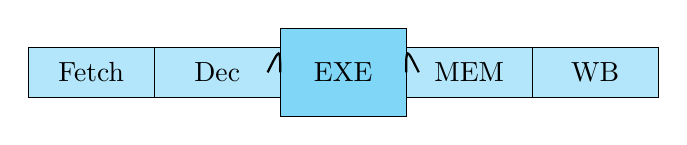
\begin{tikzpicture}[scale=0.8]
      % Single pipeline with bulge at EXE
      \draw[fill=cyan!30] (0,0) rectangle (2,0.8) node[midway] {Fetch};
      \draw[fill=cyan!30] (2,0) rectangle (4,0.8) node[midway] {Dec};
      \draw[fill=cyan!50] (4,-0.3) rectangle (6,1.1);
      \node at (5,0.4) {EXE};
      \draw[fill=cyan!30] (6,0) rectangle (8,0.8) node[midway] {MEM};
      \draw[fill=cyan!30] (8,0) rectangle (10,0.8) node[midway] {WB};
      
      % Curved lines showing bottleneck
      \draw[thick] (3.8,0.4) .. controls (4,0.8) and (4,0.8) .. (4,0.4);
      \draw[thick] (6,0.4) .. controls (6,0.8) and (6,0.8) .. (6.2,0.4);
    \end{tikzpicture}
  \end{center}
  
  \vspace{0.3cm}
  \begin{itemize}
    \item \textbf{Getting IPC $> 1$ requires to fetch, decode, exe, and retire $>1$ instruction per clock:}
  \end{itemize}
  
  \begin{center}
    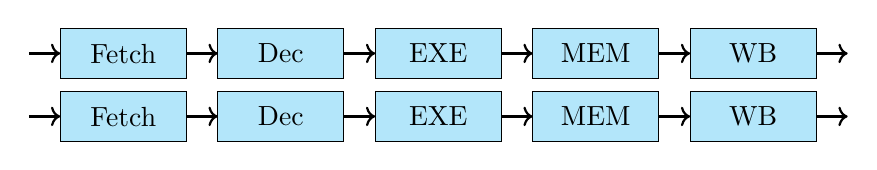
\begin{tikzpicture}[scale=0.8]
      % Dual pipeline
      \foreach \y in {0, -1} {
        \draw[->, thick] (-0.5,\y+0.4) -- (0,\y+0.4);
        \draw[fill=cyan!30] (0,\y) rectangle (2,\y+0.8) node[midway] {Fetch};
        \draw[->, thick] (2,\y+0.4) -- (2.5,\y+0.4);
        \draw[fill=cyan!30] (2.5,\y) rectangle (4.5,\y+0.8) node[midway] {Dec};
        \draw[->, thick] (4.5,\y+0.4) -- (5,\y+0.4);
        \draw[fill=cyan!30] (5,\y) rectangle (7,\y+0.8) node[midway] {EXE};
        \draw[->, thick] (7,\y+0.4) -- (7.5,\y+0.4);
        \draw[fill=cyan!30] (7.5,\y) rectangle (9.5,\y+0.8) node[midway] {MEM};
        \draw[->, thick] (9.5,\y+0.4) -- (10,\y+0.4);
        \draw[fill=cyan!30] (10,\y) rectangle (12,\y+0.8) node[midway] {WB};
        \draw[->, thick] (12,\y+0.4) -- (12.5,\y+0.4);
      }
    \end{tikzpicture}
  \end{center}
\end{frame}

\begin{frame}{The Pentium® Processor (1993)}
  \begin{itemize}
    \item \textbf{Fetch and decode 2 instructions per cycle}
    
    \item \textbf{At decode stage decide on \emph{pairing}:} can the two instructions be executed in parallel
    
    \item \textbf{Pairing decision is based on:}
    \begin{itemize}
      \item \textcolor{blue}{Data dependencies}: 2nd instruction must be independent of 1st
      \begin{itemize}
        \item If the 1st instruction produces data needed by the 2nd instruction, the 2nd instruction cannot be executed in parallel to the 1st instruction
      \end{itemize}
      
      \item \textcolor{blue}{Resources}: U-pipe and V-pipe are not symmetric (save HW)
      \begin{itemize}
        \item Common instructions can execute on either pipe
        \item Some instructions can execute only on the U-pipe
        \item V-pipe can run a subset of the instructions that can run on U-pipe
        \item If the 2nd instruction requires the U-pipe, it cannot pair
        \item Some instructions use resources of both pipes (and therefore cannot pair)
      \end{itemize}
    \end{itemize}
  \end{itemize}
  
  \begin{center}
    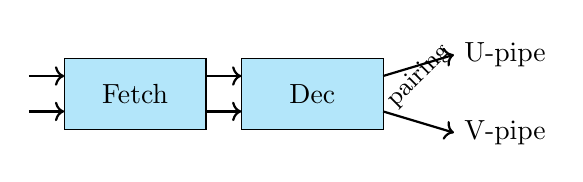
\begin{tikzpicture}[scale=0.9]
      \draw[->, thick] (-0.5,0) -- (0,0);
      \draw[->, thick] (-0.5,-0.5) -- (0,-0.5);
      \draw[fill=cyan!30] (0,-0.75) rectangle (2,0.25) node[midway] {Fetch};
      \draw[->, thick] (2,0) -- (2.5,0);
      \draw[->, thick] (2,-0.5) -- (2.5,-0.5);
      \draw[fill=cyan!30] (2.5,-0.75) rectangle (4.5,0.25) node[midway] {Dec};
      \node[rotate=45] at (5,0) {\small pairing};
      \draw[->, thick] (4.5,0) -- (5.5,0.3) node[right] {U-pipe};
      \draw[->, thick] (4.5,-0.5) -- (5.5,-0.8) node[right] {V-pipe};
    \end{tikzpicture}
  \end{center}
\end{frame}

\begin{frame}{Misprediction Penalty in a Superscalar CPU}
  \begin{itemize}
    \item \textbf{Assume}
    \begin{itemize}
      \item $\frac{1}{100}$ instruction is a mispredicted jump (MPI = 1\%)
      \item Flush penalty of 5 cycles
    \end{itemize}
    
    \vspace{0.5cm}
    
    \item \textbf{For IPC = 2}
    \begin{itemize}
      \item Flush every $\frac{100}{2} = 50$ cycles
      \item 5 cycles flush penalty every 50 cycles $\Rightarrow$ \alert{10\% performance hit}
    \end{itemize}
    
    \vspace{0.5cm}
    
    \item \textbf{For IPC = 1}
    \begin{itemize}
      \item Flush every $\frac{100}{1} = 100$ cycles
      \item 5 cycles flush penalty per 100 cycles $\Rightarrow$ \alert{5\% performance hit}
    \end{itemize}
    
    \vspace{0.5cm}
    
    \item \alert{Flush penalty increases as the machine is deeper and wider}
  \end{itemize}
\end{frame}

\begin{frame}{Extract More ILP}
  \begin{itemize}
    \item \textbf{ILP -- Instruction Level Parallelism}
    \begin{itemize}
      \item A given program, executed on a given input data has a given parallelism
      \item Can execute only independent instructions in parallel
      \item If for example each instruction is dependent on the previous instruction, ILP = 1
      \begin{itemize}
        \item Adding more HW will not change that
      \end{itemize}
    \end{itemize}
    
    \item \textbf{Adjacent instructions are usually dependent}
    \begin{itemize}
      \item 2nd pipe utilization is lower than 1st pipe utilization, a 3rd pipe utilization further goes down
    \end{itemize}
    
    \item \textbf{Cache misses stall execution} -- instructions dependent on a missed load stall
    
    \item \textbf{Compilers are limited to basic blocks}, and are not aware of cache misses
    
    \item \textbf{Solution: Out-Of-Order Execution}
    \begin{itemize}
      \item Look for independent instructions further ahead in the program
      \item Execute instructions based on data readiness
      \item Still need to keep the semantics of the original program
    \end{itemize}
  \end{itemize}
\end{frame}

\begin{frame}{Data Flow Analysis}
  \begin{columns}
    \begin{column}{0.35\textwidth}
      \textbf{Example:}
      \begin{enumerate}
        \item \texttt{\textcolor{r1color}{r1} $\leftarrow$ r4 / r7}
        \item \texttt{\textcolor{r8color}{r8} $\leftarrow$ \textcolor{r1color}{r1} + r2}
        \item \texttt{\textcolor{r5color}{r5} $\leftarrow$ r5 + 1}
        \item \texttt{\textcolor{r6color}{r6} $\leftarrow$ r6 - r3}
        \item \texttt{\textcolor{r4color}{r4} $\leftarrow$ \textcolor{r5color}{r5} + \textcolor{r6color}{r6}}
        \item \texttt{r7 $\leftarrow$ \textcolor{r8color}{r8} * \textcolor{r4color}{r4}}
      \end{enumerate}
      
      \vspace{0.3cm}
      \small{Assume divide takes multiple cycles}
    \end{column}
    
    \begin{column}{0.65\textwidth}
      \begin{center}
        \textbf{Data Flow Graph}\\
        \vspace{0.3cm}
        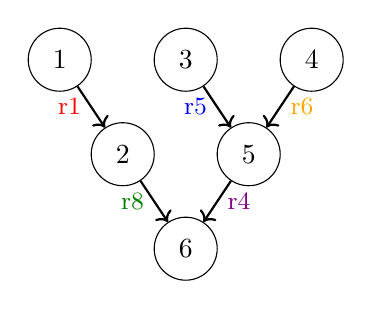
\begin{tikzpicture}[scale=0.8, 
          node distance=1.2cm,
          inst/.style={circle, draw, minimum size=0.8cm},
          dep/.style={->, thick}]
          
          % Nodes
          \node[inst] (i1) at (0,2.5) {1};
          \node[inst] (i3) at (2,2.5) {3};
          \node[inst] (i4) at (4,2.5) {4};
          \node[inst] (i2) at (1,1) {2};
          \node[inst] (i5) at (3,1) {5};
          \node[inst] (i6) at (2,-0.5) {6};
          
          % Dependencies with colored labels
          \draw[dep] (i1) -- node[left] {\textcolor{r1color}{\small r1}} (i2);
          \draw[dep] (i3) -- node[left] {\textcolor{r5color}{\small r5}} (i5);
          \draw[dep] (i4) -- node[right] {\textcolor{r6color}{\small r6}} (i5);
          \draw[dep] (i2) -- node[left] {\textcolor{r8color}{\small r8}} (i6);
          \draw[dep] (i5) -- node[right] {\textcolor{r4color}{\small r4}} (i6);
        \end{tikzpicture}
        
        \vspace{0.5cm}
        \small
        \begin{tabular}{cc}
          \textbf{In-order execution} & \textbf{Out-of-order execution} \\
        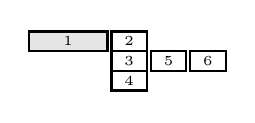
\begin{tikzpicture}[scale=0.5]
        % Box 1 (large, left side)
        \draw[thick, fill=gray!20] (0,1) rectangle (2,1.5) node[midway, font=\tiny] {1};
        
        % Box 2 (top right)
        \draw[thick, fill=white] (2.1,1) rectangle (3,1.5) node[midway, font=\tiny] {2};
        
        % Box 3 (middle right)
        \draw[thick, fill=white] (2.1,0.5) rectangle (3,1) node[midway, font=\tiny] {3};
        
        % Box 4 (bottom middle)
        \draw[thick, fill=white] (2.1,0) rectangle (3,0.5) node[midway, font=\tiny] {4};
        
        % Box 5 (right of box 3)
        \draw[thick, fill=white] (3.1,0.5) rectangle (4,1) node[midway, font=\tiny] {5};
        
        % Box 6 (far right)
        \draw[thick, fill=white] (4.1,0.5) rectangle (5,1) node[midway, font=\tiny] {6};
        \end{tikzpicture}
          &
          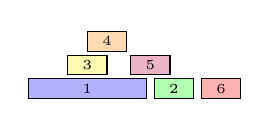
\begin{tikzpicture}[scale=0.5]
            \draw[fill=blue!30] (0,0) rectangle (3,0.5) node[midway] {\tiny 1};
            \draw[fill=yellow!30] (1,0.6) rectangle (2,1.1) node[midway] {\tiny 3};
            \draw[fill=orange!30] (1.5,1.2) rectangle (2.5,1.7) node[midway] {\tiny 4};
            \draw[fill=purple!30] (2.6,0.6) rectangle (3.6,1.1) node[midway] {\tiny 5};
            \draw[fill=green!30] (3.2,0) rectangle (4.2,0.5) node[midway] {\tiny 2};
            \draw[fill=red!30] (4.4,0) rectangle (5.4,0.5) node[midway] {\tiny 6};
          \end{tikzpicture}
        \end{tabular}
      \end{center}
    \end{column}
  \end{columns}
\end{frame}

\begin{frame}{OOOE -- General Scheme}
  \begin{center}
    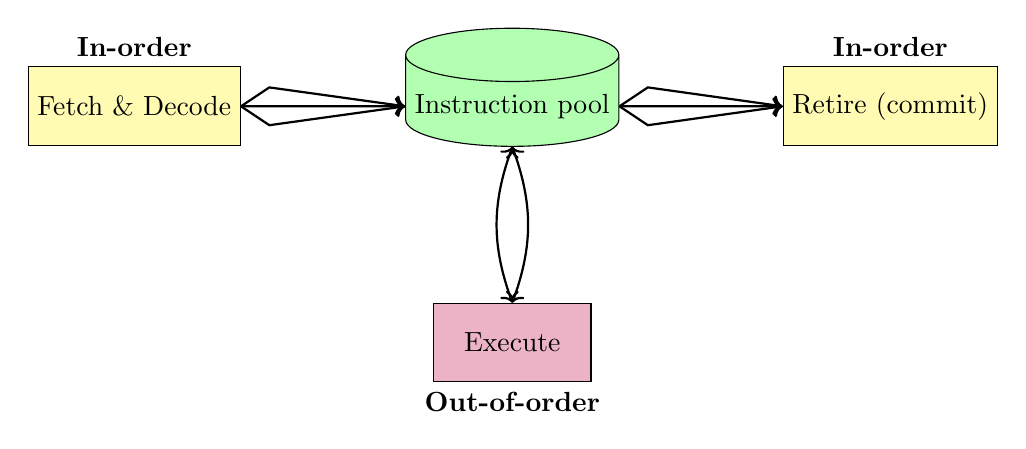
\begin{tikzpicture}[scale=1.2,
      block/.style={rectangle, draw, fill=yellow!30, minimum width=2.5cm, minimum height=1cm},
      pool/.style={cylinder, draw, fill=green!30, minimum width=2cm, minimum height=1.5cm, shape border rotate=90, aspect=0.25},
      exe/.style={rectangle, draw, fill=purple!30, minimum width=2cm, minimum height=1cm}]
      
      % Blocks
      \node[block] (fetch) at (0,0) {Fetch \& Decode};
      \node[pool] (pool) at (4,0) {Instruction pool};
      \node[exe] (exec) at (4,-2.5) {Execute};
      \node[block] (retire) at (8,0) {Retire (commit)};
      
      % Arrows with multiple lines
      \foreach \y in {-0.2, 0, 0.2} {
        \draw[->, thick] (fetch.east) -- ++(0.3,\y) -- (pool.west);
        \draw[->, thick] (pool.east) -- ++(0.3,\y) -- (retire.west);
      }
      
      % Bidirectional connection pool-execute
      \draw[<->, thick, bend right=20] (pool.south) to (exec.north);
      \draw[<->, thick, bend left=20] (pool.south) to (exec.north);
      
      % Labels
      \node[above] at (fetch.north) {\textbf{In-order}};
      \node[above] at (retire.north) {\textbf{In-order}};
      \node[below] at (exec.south) {\textbf{Out-of-order}};
    \end{tikzpicture}
  \end{center}
  
  \vspace{0.5cm}
  
  \begin{itemize}
    \item \textbf{Fetch \& decode instructions in parallel but in-order}
    \begin{itemize}
      \item Fill the Instruction Pool
    \end{itemize}
    
    \item \textbf{Execute ready instructions from the instructions pool}
    \begin{itemize}
      \item All source data ready + needed execution resources available
    \end{itemize}
    
    \item \textbf{Once an instruction is executed}
    \begin{itemize}
      \item Signal all dependent instructions that data is ready
    \end{itemize}
    
    \item \textbf{Commit instructions in parallel but in-order}
    \begin{itemize}
      \item State change (memory, register) and fault/exception handling
    \end{itemize}
  \end{itemize}
\end{frame}

\begin{frame}{Write-After-Write Dependency}
  \begin{columns}
    \begin{column}{0.5\textwidth}
      \textbf{Example Code:} \\
      \begin{tabular}{lll}
        (1) & & \texttt{\textcolor{r1color}{r1} $\leftarrow$ r9/17} \\
        (2) & & \texttt{\textcolor{r2color}{r2} $\leftarrow$ \textcolor{r2color}{r2}+\textcolor{r1color}{r1}} \\
        (3) & & \texttt{\textcolor{orange}{r1} $\leftarrow$ 23} \\
        (4) & & \texttt{\textcolor{r3color}{r3} $\leftarrow$ \textcolor{r3color}{r3}+\textcolor{orange}{r1}} \\
        (5) & & \texttt{jcc L2} \\
        (6) & \texttt{L2:} & \texttt{\textcolor{green}{r1} $\leftarrow$ 35} \\
        (7) & & \texttt{\textcolor{r4color}{r4} $\leftarrow$ \textcolor{r3color}{r3}+\textcolor{green}{r1}} \\
        (8) & & \texttt{\textcolor{blue}{r3} $\leftarrow$ 2} \\
      \end{tabular}
    \end{column}
    
    \begin{column}{0.5\textwidth}
      \begin{block}{WAW Issue}
        If inst (3) is executed before inst (1), r1 ends up having a wrong value.
        
        \vspace{0.3cm}
        
        Called \alert{write-after-write false dependency}:
        
        The order of two writes to the same register is flipped.
      \end{block}
    \end{column}
  \end{columns}
\end{frame}
\begin{frame}{What's Next}
  \begin{itemize}
    \item \textbf{Goal: minimize CPU Time}
    \begin{equation*}
      \text{CPU Time} = \text{clock cycle} \times \text{CPI} \times \text{IC}
    \end{equation*}
    
    \item \textbf{So far we have learned}
    \begin{itemize}
      \item Minimize clock cycle $\Rightarrow$ add more pipe stages
      \item Minimize CPI $\Rightarrow$ use pipeline
      \item Minimize IC $\Rightarrow$ architecture
    \end{itemize}
    
    \item \textbf{In a pipelined CPU}
    \begin{itemize}
      \item CPI w/o hazards is 1
      \item CPI with hazards is $> 1$
    \end{itemize}
    
    \item \textbf{Adding more pipe stages reduces clock cycle but increases CPI}
    \begin{itemize}
      \item Higher penalty due to control hazards
      \item More data hazards
    \end{itemize}
    
    \item \alert{What can we do? Further reduce the CPI!}
  \end{itemize}
\end{frame}

\begin{frame}{A Superscalar CPU}
  \begin{itemize}
    \item \textbf{Duplicating HW in one pipe stage won't help}
    \begin{itemize}
      \item e.g., have 2 ALUs
      \item the bottleneck moves to other stages
    \end{itemize}
  \end{itemize}
  
  \begin{center}
    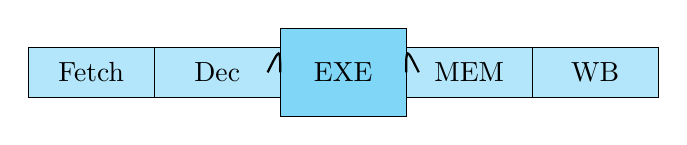
\begin{tikzpicture}[scale=0.8]
      % Single pipeline with bulge at EXE
      \draw[fill=cyan!30] (0,0) rectangle (2,0.8) node[midway] {Fetch};
      \draw[fill=cyan!30] (2,0) rectangle (4,0.8) node[midway] {Dec};
      \draw[fill=cyan!50] (4,-0.3) rectangle (6,1.1);
      \node at (5,0.4) {EXE};
      \draw[fill=cyan!30] (6,0) rectangle (8,0.8) node[midway] {MEM};
      \draw[fill=cyan!30] (8,0) rectangle (10,0.8) node[midway] {WB};
      
      % Curved lines showing bottleneck
      \draw[thick] (3.8,0.4) .. controls (4,0.8) and (4,0.8) .. (4,0.4);
      \draw[thick] (6,0.4) .. controls (6,0.8) and (6,0.8) .. (6.2,0.4);
    \end{tikzpicture}
  \end{center}
  
  \vspace{0.3cm}
  \begin{itemize}
    \item \textbf{Getting IPC $> 1$ requires to fetch, decode, exe, and retire $>1$ instruction per clock:}
  \end{itemize}
  
  \begin{center}
    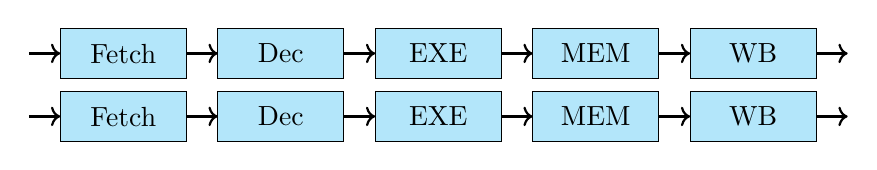
\begin{tikzpicture}[scale=0.8]
      % Dual pipeline
      \foreach \y in {0, -1} {
        \draw[->, thick] (-0.5,\y+0.4) -- (0,\y+0.4);
        \draw[fill=cyan!30] (0,\y) rectangle (2,\y+0.8) node[midway] {Fetch};
        \draw[->, thick] (2,\y+0.4) -- (2.5,\y+0.4);
        \draw[fill=cyan!30] (2.5,\y) rectangle (4.5,\y+0.8) node[midway] {Dec};
        \draw[->, thick] (4.5,\y+0.4) -- (5,\y+0.4);
        \draw[fill=cyan!30] (5,\y) rectangle (7,\y+0.8) node[midway] {EXE};
        \draw[->, thick] (7,\y+0.4) -- (7.5,\y+0.4);
        \draw[fill=cyan!30] (7.5,\y) rectangle (9.5,\y+0.8) node[midway] {MEM};
        \draw[->, thick] (9.5,\y+0.4) -- (10,\y+0.4);
        \draw[fill=cyan!30] (10,\y) rectangle (12,\y+0.8) node[midway] {WB};
        \draw[->, thick] (12,\y+0.4) -- (12.5,\y+0.4);
      }
    \end{tikzpicture}
  \end{center}
\end{frame}

\begin{frame}{The Pentium® Processor (1993)}
  \begin{itemize}
    \item \textbf{Fetch and decode 2 instructions per cycle}
    
    \item \textbf{At decode stage decide on \emph{pairing}:} can the two instructions be executed in parallel
    
    \item \textbf{Pairing decision is based on:}
    \begin{itemize}
      \item \textcolor{blue}{Data dependencies}: 2nd instruction must be independent of 1st
      \begin{itemize}
        \item If the 1st instruction produces data needed by the 2nd instruction, the 2nd instruction cannot be executed in parallel to the 1st instruction
      \end{itemize}
      
      \item \textcolor{blue}{Resources}: U-pipe and V-pipe are not symmetric (save HW)
      \begin{itemize}
        \item Common instructions can execute on either pipe
        \item Some instructions can execute only on the U-pipe
        \item V-pipe can run a subset of the instructions that can run on U-pipe
        \item If the 2nd instruction requires the U-pipe, it cannot pair
        \item Some instructions use resources of both pipes (and therefore cannot pair)
      \end{itemize}
    \end{itemize}
  \end{itemize}
  
  \begin{center}
    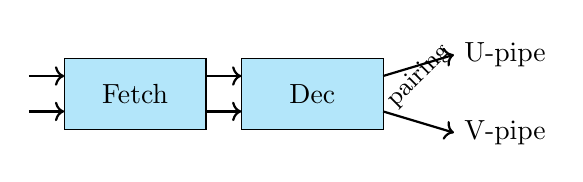
\begin{tikzpicture}[scale=0.9]
      \draw[->, thick] (-0.5,0) -- (0,0);
      \draw[->, thick] (-0.5,-0.5) -- (0,-0.5);
      \draw[fill=cyan!30] (0,-0.75) rectangle (2,0.25) node[midway] {Fetch};
      \draw[->, thick] (2,0) -- (2.5,0);
      \draw[->, thick] (2,-0.5) -- (2.5,-0.5);
      \draw[fill=cyan!30] (2.5,-0.75) rectangle (4.5,0.25) node[midway] {Dec};
      \node[rotate=45] at (5,0) {\small pairing};
      \draw[->, thick] (4.5,0) -- (5.5,0.3) node[right] {U-pipe};
      \draw[->, thick] (4.5,-0.5) -- (5.5,-0.8) node[right] {V-pipe};
    \end{tikzpicture}
  \end{center}
\end{frame}

\begin{frame}{Misprediction Penalty in a Superscalar CPU}
  \begin{itemize}
    \item \textbf{Assume}
    \begin{itemize}
      \item $\frac{1}{100}$ instruction is a mispredicted jump (MPI = 1\%)
      \item Flush penalty of 5 cycles
    \end{itemize}
    
    \vspace{0.5cm}
    
    \item \textbf{For IPC = 2}
    \begin{itemize}
      \item Flush every $\frac{100}{2} = 50$ cycles
      \item 5 cycles flush penalty every 50 cycles $\Rightarrow$ \alert{10\% performance hit}
    \end{itemize}
    
    \vspace{0.5cm}
    
    \item \textbf{For IPC = 1}
    \begin{itemize}
      \item Flush every $\frac{100}{1} = 100$ cycles
      \item 5 cycles flush penalty per 100 cycles $\Rightarrow$ \alert{5\% performance hit}
    \end{itemize}
    
    \vspace{0.5cm}
    
    \item \alert{Flush penalty increases as the machine is deeper and wider}
  \end{itemize}
\end{frame}

\begin{frame}{Extract More ILP}
  \begin{itemize}
    \item \textbf{ILP -- Instruction Level Parallelism}
    \begin{itemize}
      \item A given program, executed on a given input data has a given parallelism
      \item Can execute only independent instructions in parallel
      \item If for example each instruction is dependent on the previous instruction, ILP = 1
      \begin{itemize}
        \item Adding more HW will not change that
      \end{itemize}
    \end{itemize}
    
    \item \textbf{Adjacent instructions are usually dependent}
    \begin{itemize}
      \item 2nd pipe utilization is lower than 1st pipe utilization, a 3rd pipe utilization further goes down
    \end{itemize}
    
    \item \textbf{Cache misses stall execution} -- instructions dependent on a missed load stall
    
    \item \textbf{Compilers are limited to basic blocks}, and are not aware of cache misses
    
    \item \textbf{Solution: Out-Of-Order Execution}
    \begin{itemize}
      \item Look for independent instructions further ahead in the program
      \item Execute instructions based on data readiness
      \item Still need to keep the semantics of the original program
    \end{itemize}
  \end{itemize}
\end{frame}

\begin{frame}{Data Flow Analysis}
  \begin{columns}
    \begin{column}{0.35\textwidth}
      \textbf{Example:}
      \begin{enumerate}
        \item \texttt{\textcolor{r1color}{r1} $\leftarrow$ r4 / r7}
        \item \texttt{\textcolor{r8color}{r8} $\leftarrow$ \textcolor{r1color}{r1} + r2}
        \item \texttt{\textcolor{r5color}{r5} $\leftarrow$ r5 + 1}
        \item \texttt{\textcolor{r6color}{r6} $\leftarrow$ r6 - r3}
        \item \texttt{\textcolor{r4color}{r4} $\leftarrow$ \textcolor{r5color}{r5} + \textcolor{r6color}{r6}}
        \item \texttt{r7 $\leftarrow$ \textcolor{r8color}{r8} * \textcolor{r4color}{r4}}
      \end{enumerate}
      
      \vspace{0.3cm}
      \small{Assume divide takes multiple cycles}
    \end{column}
    
    \begin{column}{0.65\textwidth}
      \begin{center}
        \textbf{Data Flow Graph}\\
        \vspace{0.3cm}
        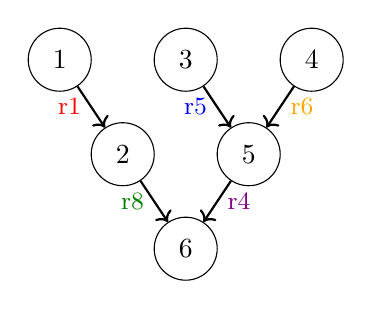
\begin{tikzpicture}[scale=0.8, 
          node distance=1.2cm,
          inst/.style={circle, draw, minimum size=0.8cm},
          dep/.style={->, thick}]
          
          % Nodes
          \node[inst] (i1) at (0,2.5) {1};
          \node[inst] (i3) at (2,2.5) {3};
          \node[inst] (i4) at (4,2.5) {4};
          \node[inst] (i2) at (1,1) {2};
          \node[inst] (i5) at (3,1) {5};
          \node[inst] (i6) at (2,-0.5) {6};
          
          % Dependencies with colored labels
          \draw[dep] (i1) -- node[left] {\textcolor{r1color}{\small r1}} (i2);
          \draw[dep] (i3) -- node[left] {\textcolor{r5color}{\small r5}} (i5);
          \draw[dep] (i4) -- node[right] {\textcolor{r6color}{\small r6}} (i5);
          \draw[dep] (i2) -- node[left] {\textcolor{r8color}{\small r8}} (i6);
          \draw[dep] (i5) -- node[right] {\textcolor{r4color}{\small r4}} (i6);
        \end{tikzpicture}
        
        \vspace{0.5cm}
        \small
        \begin{tabular}{cc}
          \textbf{In-order execution} & \textbf{Out-of-order execution} \\
        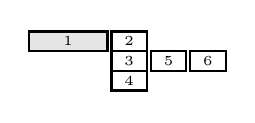
\begin{tikzpicture}[scale=0.5]
        % Box 1 (large, left side)
        \draw[thick, fill=gray!20] (0,1) rectangle (2,1.5) node[midway, font=\tiny] {1};
        
        % Box 2 (top right)
        \draw[thick, fill=white] (2.1,1) rectangle (3,1.5) node[midway, font=\tiny] {2};
        
        % Box 3 (middle right)
        \draw[thick, fill=white] (2.1,0.5) rectangle (3,1) node[midway, font=\tiny] {3};
        
        % Box 4 (bottom middle)
        \draw[thick, fill=white] (2.1,0) rectangle (3,0.5) node[midway, font=\tiny] {4};
        
        % Box 5 (right of box 3)
        \draw[thick, fill=white] (3.1,0.5) rectangle (4,1) node[midway, font=\tiny] {5};
        
        % Box 6 (far right)
        \draw[thick, fill=white] (4.1,0.5) rectangle (5,1) node[midway, font=\tiny] {6};
        \end{tikzpicture}
          &
          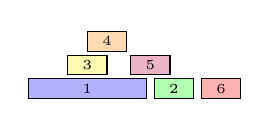
\begin{tikzpicture}[scale=0.5]
            \draw[fill=blue!30] (0,0) rectangle (3,0.5) node[midway] {\tiny 1};
            \draw[fill=yellow!30] (1,0.6) rectangle (2,1.1) node[midway] {\tiny 3};
            \draw[fill=orange!30] (1.5,1.2) rectangle (2.5,1.7) node[midway] {\tiny 4};
            \draw[fill=purple!30] (2.6,0.6) rectangle (3.6,1.1) node[midway] {\tiny 5};
            \draw[fill=green!30] (3.2,0) rectangle (4.2,0.5) node[midway] {\tiny 2};
            \draw[fill=red!30] (4.4,0) rectangle (5.4,0.5) node[midway] {\tiny 6};
          \end{tikzpicture}
        \end{tabular}
      \end{center}
    \end{column}
  \end{columns}
\end{frame}

\begin{frame}{OOOE -- General Scheme}
  \begin{center}
    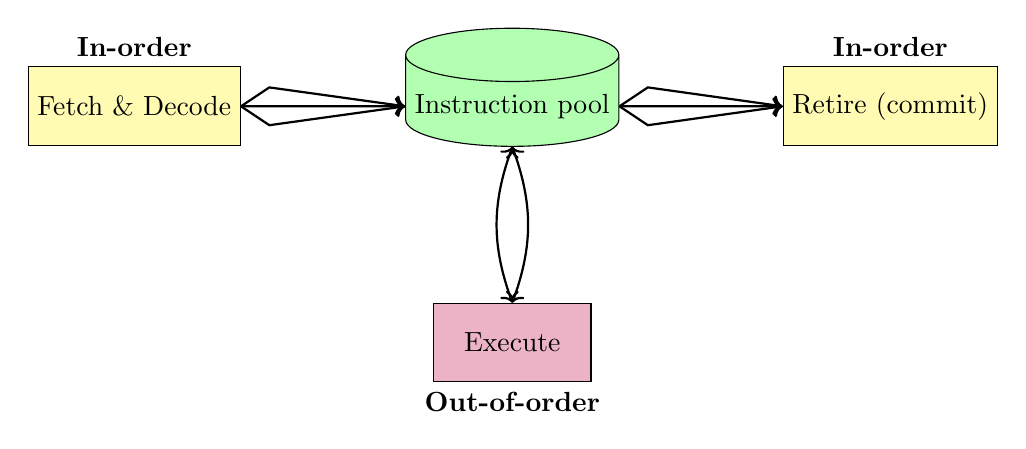
\begin{tikzpicture}[scale=1.2,
      block/.style={rectangle, draw, fill=yellow!30, minimum width=2.5cm, minimum height=1cm},
      pool/.style={cylinder, draw, fill=green!30, minimum width=2cm, minimum height=1.5cm, shape border rotate=90, aspect=0.25},
      exe/.style={rectangle, draw, fill=purple!30, minimum width=2cm, minimum height=1cm}]
      
      % Blocks
      \node[block] (fetch) at (0,0) {Fetch \& Decode};
      \node[pool] (pool) at (4,0) {Instruction pool};
      \node[exe] (exec) at (4,-2.5) {Execute};
      \node[block] (retire) at (8,0) {Retire (commit)};
      
      % Arrows with multiple lines
      \foreach \y in {-0.2, 0, 0.2} {
        \draw[->, thick] (fetch.east) -- ++(0.3,\y) -- (pool.west);
        \draw[->, thick] (pool.east) -- ++(0.3,\y) -- (retire.west);
      }
      
      % Bidirectional connection pool-execute
      \draw[<->, thick, bend right=20] (pool.south) to (exec.north);
      \draw[<->, thick, bend left=20] (pool.south) to (exec.north);
      
      % Labels
      \node[above] at (fetch.north) {\textbf{In-order}};
      \node[above] at (retire.north) {\textbf{In-order}};
      \node[below] at (exec.south) {\textbf{Out-of-order}};
    \end{tikzpicture}
  \end{center}
  
  \vspace{0.5cm}
  
  \begin{itemize}
    \item \textbf{Fetch \& decode instructions in parallel but in-order}
    \begin{itemize}
      \item Fill the Instruction Pool
    \end{itemize}
    
    \item \textbf{Execute ready instructions from the instructions pool}
    \begin{itemize}
      \item All source data ready + needed execution resources available
    \end{itemize}
    
    \item \textbf{Once an instruction is executed}
    \begin{itemize}
      \item Signal all dependent instructions that data is ready
    \end{itemize}
    
    \item \textbf{Commit instructions in parallel but in-order}
    \begin{itemize}
      \item State change (memory, register) and fault/exception handling
    \end{itemize}
  \end{itemize}
\end{frame}

\begin{frame}{Write-After-Write Dependency}
  \begin{columns}
    \begin{column}{0.5\textwidth}
      \textbf{Example Code:} \\
      \begin{tabular}{lll}
        (1) & & \texttt{\textcolor{blue}{r1} $\leftarrow$ r9/17} \\
        (2) & & \texttt{r2 $\leftarrow$ r2+\textcolor{blue}{r1}} \\
        (3) & & \texttt{\textcolor{orange}{r1} $\leftarrow$ 23} \\
        (4) & & \texttt{r3 $\leftarrow$ r3+\textcolor{orange}{r1}} \\
        (5) & & \texttt{jcc L2} \\
        (6) & \texttt{L2:} & \texttt{\textcolor{green}{r1} $\leftarrow$ 35} \\
        (7) & & \texttt{r4 $\leftarrow$ r3+\textcolor{green}{r1}} \\
        (8) & & \texttt{r3 $\leftarrow$ 2} \\
      \end{tabular}
    \end{column}
    
    \begin{column}{0.5\textwidth}
      \begin{block}{WAW Issue}
        If inst (3) is executed before inst (1), r1 ends up having a wrong value.
        
        \vspace{0.3cm}
        
        Called \alert{write-after-write false dependency}:
        
        The order of two writes to the same register is flipped.
      \end{block}
    \end{column}
  \end{columns}
\end{frame}

\begin{frame}{Write-After-Write Dependency}
  \begin{columns}
    \begin{column}{0.5\textwidth}
      \textbf{Example Code (reordered):} \\
      \begin{tabular}{lll}
        (3) & & \texttt{\textcolor{orange}{r1} $\leftarrow$ 23} \\
        (1) & & \texttt{\textcolor{blue}{r1} $\leftarrow$ r9/17} \\
        (2) & & \texttt{r2 $\leftarrow$ r2+\textcolor{blue}{r1}} \\
        & & \\
        (4) & & \texttt{r3 $\leftarrow$ r3+\textcolor{orange}{r1}} \\
        (5) & & \texttt{jcc L2} \\
        (6) & \texttt{L2:} & \texttt{\textcolor{green}{r1} $\leftarrow$ 35} \\
        (7) & & \texttt{r4 $\leftarrow$ r3+\textcolor{green}{r1}} \\
        (8) & & \texttt{r3 $\leftarrow$ 2} \\
      \end{tabular}
    \end{column}
    
    \begin{column}{0.5\textwidth}
      \begin{block}{Correct Dependency}
        Inst (4) should use the value of \textcolor{orange}{r1} produced by inst (3), even if inst (1) is executed after inst (3).
        
        \vspace{0.3cm}
        
        \alert{Write-After-Write (WAW) is a \emph{false dependency}}
        
        Not a real data dependency, but an artifact of OOO execution
      \end{block}
      
      % Arrow showing dependency
      \begin{tikzpicture}[overlay, remember picture]
        \draw[->, thick, orange, dashed] (-4.5,1.8) -- (-2.8,0.8);
      \end{tikzpicture}
    \end{column}
  \end{columns}
\end{frame}

\begin{frame}{Speculative Execution}
  \begin{columns}
    \begin{column}{0.45\textwidth}
      \textbf{Example Code:} \\
      \begin{tabular}{lll}
        (3) & & \texttt{\textcolor{orange}{r1} $\leftarrow$ 23} \\
        (1) & & \texttt{\textcolor{blue}{r1} $\leftarrow$ r9/17} \\
        (2) & & \texttt{r2 $\leftarrow$ r2+\textcolor{blue}{r1}} \\
        (4) & & \texttt{r3 $\leftarrow$ r3+\textcolor{orange}{r1}} \\
        (5) & & \texttt{jcc L2} \\
        \rowcolor{pink!30} (6) & \texttt{L2:} & \texttt{\textcolor{green}{r1} $\leftarrow$ 35} \\
        \rowcolor{pink!30} (7) & & \texttt{r4 $\leftarrow$ r3+\textcolor{green}{r1}} \\
        \rowcolor{pink!30} (8) & & \texttt{r3 $\leftarrow$ 2} \\
      \end{tabular}
    \end{column}
    
    \begin{column}{0.55\textwidth}
      \begin{block}{OOO Speculative Execution}
        \small
        \textbf{Every 5th instruction is a branch} $\Rightarrow$ must continue fetching along \textcolor{green}{predicted path} to fill instruction pool.
        
        Without speculation: limited to finding independent instructions only until next branch.
        
        \alert{Speculative Execution:} Execute instructions from predicted path before branch resolution.
        
        Example: inst (6) can execute before inst (1).
        
        If mispredicted: must undo speculatively executed instructions.
      \end{block}
    \end{column}
  \end{columns}
\end{frame}

\begin{frame}{Write-After-Read Dependency}
  \begin{columns}
    \begin{column}{0.5\textwidth}
      \textbf{Example Code:} \\
      \begin{tabular}{lll}
        (3) & & \texttt{\textcolor{orange}{r1} $\leftarrow$ 23} \\
        (1) & & \texttt{\textcolor{blue}{r1} $\leftarrow$ r9/17} \\
        (2) & & \texttt{r2 $\leftarrow$ r2+\textcolor{blue}{r1}} \\
        & & \\
        (4) & & \texttt{r3 $\leftarrow$ r3+\textcolor{orange}{r1}} \\
        (5) & & \texttt{jcc L2} \\
        (6) & \texttt{L2:} & \texttt{\textcolor{green}{r1} $\leftarrow$ 35} \\
        (8) & & \texttt{\textcolor{blue}{r3} $\leftarrow$ 2} \\
        (7) & & \texttt{r4 $\leftarrow$ \textcolor{red}{r3}+\textcolor{green}{r1}} \\
      \end{tabular}
    \end{column}
    
    \begin{column}{0.5\textwidth}
      \begin{block}{WAR Issue}
        If inst (8) is executed before inst (7), inst (7) gets a wrong value of r3.
        
        \vspace{0.3cm}
        
        Called \alert{write-after-read false dependency}.
        
        \vspace{0.3cm}
        
        \alert{Write-After-Read (WAR) is a \emph{false dependency}}
        
        Not a real data dependency, but an artifact of OOO execution
      \end{block}
      
      % Arrow showing dependency
      \begin{tikzpicture}[overlay, remember picture]
        \draw[->, thick, red, dashed] (-2.5,-0.4) -- (-4,-1.2);
      \end{tikzpicture}
    \end{column}
  \end{columns}
\end{frame}

\begin{frame}{Register Renaming}
  \begin{itemize}
    \item \textbf{Hold a pool of \emph{physical registers}}
    \begin{itemize}
      \item Maintain a mapping of architectural registers to physical registers
    \end{itemize}
    
    \item \textbf{When an instruction is allocated into the instruction pool (in-order)}
    \begin{enumerate}
      \item If the instruction writes to a destination register Rx, map Rx to a free physical register from a pool, PRi
      \item Update the mapping of Rx to Pri: the latest value for Rx is stored in PRi
      \item Rename the architectural source registers of the instruction with the currently mapped physical registers (or arch register if no physical register)
    \end{enumerate}
    
    \item \textbf{Send instruction to EXE (out-of-order)}
    \begin{itemize}
      \item When its physical sources are ready AND needed execution resources are available
      \item The instruction uses the correct sources, regardless of the execution order
      \item Instead of writing the result to Rx, the instruction writes the result to PRi
    \end{itemize}
    
    \item \textbf{When an instruction commits (in-order)}
    \begin{itemize}
      \item Copy the value from its physical register to the architectural register: Rx $\leftarrow$ PRi
      \item If the current mapping of Rx is still the physical PRi (so far, no subsequent instruction writes to Rx)
      \begin{itemize}
        \item Set Rx's mapping to be architectural (the most updated value of Rx is in Rx)
      \end{itemize}
      \item Return PRi to the free physical register pool
    \end{itemize}
  \end{itemize}
\end{frame}

\begin{frame}{Register Renaming}
  \begin{columns}
    \begin{column}{0.5\textwidth}
      \begin{tabular}{lll}
        \multicolumn{3}{c}{\textbf{Original}} \\
        (1) & r1 $\leftarrow$ 17 & \\
        (2) & r2 $\leftarrow$ r2+r1 & \\
        (3) & r1 $\leftarrow$ 23 & \\
        (4) & r3 $\leftarrow$ r3+r1 & \\
        (5) & jcc L2 & \\
        (6) L2: & r1 $\leftarrow$ 35 & \\
        (7) & r4 $\leftarrow$ r3+r1 & \\
        (8) & r3 $\leftarrow$ 2 & \\
      \end{tabular}
    \end{column}
    
    \begin{column}{0.5\textwidth}
      \begin{tabular}{lll}
        \multicolumn{3}{c}{\textbf{Renaming}} \\
        r1:pr1 & pr1 $\leftarrow$ 17 & \\
        r2:pr2 & pr2 $\leftarrow$ r2+pr1 & \\
        & & \\
        & & \\
        & & \\
        & & \\
        & & \\
        & & \\
      \end{tabular}
      
      \vspace{0.5cm}
      \begin{block}{Note}
        \small
        r2 is used for both source and destination.
        This explains why first the source registers are renamed according to the current mapping, and only then the mapping of the destination register r2 is updated by the newly allocated physical register pr2.
      \end{block}
    \end{column}
  \end{columns}
  
  \vspace{0.3cm}
  \begin{center}
    \begin{tabular}{|c|c|c|c|c|}
      \hline
      & r1 & r2 & r3 & r4 \\
      \hline
      Register mapping & pr1 & pr2 & r3 & r4 \\
      \hline
    \end{tabular}
  \end{center}
\end{frame}

\begin{frame}{Register Renaming}
  \begin{columns}
    \begin{column}{0.5\textwidth}
      \begin{tabular}{lll}
        \multicolumn{3}{c}{\textbf{Original}} \\
        (1) & r1 $\leftarrow$ 17 & \\
        (2) & r2 $\leftarrow$ r2+r1 & \\
        (3) & r1 $\leftarrow$ 23 & \\
        (4) & r3 $\leftarrow$ r3+r1 & \\
        (5) & jcc L2 & \\
        (6) L2: & r1 $\leftarrow$ 35 & \\
        (7) & r4 $\leftarrow$ r3+r1 & \\
        (8) & r3 $\leftarrow$ 2 & \\
      \end{tabular}
    \end{column}
    
    \begin{column}{0.5\textwidth}
      \begin{tabular}{lll}
        \multicolumn{3}{c}{\textbf{Renaming}} \\
        r1:pr1 & pr1 $\leftarrow$ 17 & \\
        r2:pr2 & pr2 $\leftarrow$ r2+pr1 & \\
        r1:pr3 & pr3 $\leftarrow$ 23 & \\
        r3:pr4 & pr4 $\leftarrow$ r3+pr3 & \\
        & & \\
        & & \\
        & & \\
        & & \\
      \end{tabular}
    \end{column}
  \end{columns}
  
  \vspace{0.5cm}
  \begin{center}
    \begin{tabular}{|c|c|c|c|c|}
      \hline
      & r1 & r2 & r3 & r4 \\
      \hline
      Register mapping & pr3 & pr2 & pr4 & r4 \\
      \hline
    \end{tabular}
  \end{center}
  
  \begin{center}
    \colorbox{green!30}{Each instruction uses the correct sources, regardless of the execution order}
  \end{center}
\end{frame}

\begin{frame}{Register Renaming}
  \begin{columns}
    \begin{column}{0.5\textwidth}
      \begin{tabular}{lll}
        \multicolumn{3}{c}{\textbf{Original}} \\
        (1) & r1 $\leftarrow$ 17 & \\
        (2) & r2 $\leftarrow$ r2+r1 & \\
        (3) & r1 $\leftarrow$ 23 & \\
        (4) & r3 $\leftarrow$ r3+r1 & \\
        (5) & jcc L2 & \\
        (6) L2: & r1 $\leftarrow$ 35 & \\
        (7) & r4 $\leftarrow$ r3+r1 & \\
        (8) & r3 $\leftarrow$ 2 & \\
      \end{tabular}
    \end{column}
    
    \begin{column}{0.5\textwidth}
      \begin{tabular}{lll}
        \multicolumn{3}{c}{\textbf{Renaming}} \\
        r1:pr1 & pr1 $\leftarrow$ 17 & \\
        r2:pr2 & pr2 $\leftarrow$ r2+pr1 & \\
        r1:pr3 & pr3 $\leftarrow$ 23 & \\
        r3:pr4 & pr4 $\leftarrow$ r3+pr3 & \\
        & & \\
        r1:pr5 & pr5 $\leftarrow$ 35 & \\
        r4:pr6 & pr6 $\leftarrow$ pr4+pr5 & \\
        r3:pr7 & pr7 $\leftarrow$ 2 & \\
      \end{tabular}
    \end{column}
  \end{columns}
  
  \vspace{0.5cm}
  \begin{center}
    \begin{tabular}{|c|c|c|c|c|}
      \hline
      & r1 & r2 & r3 & r4 \\
      \hline
      Register mapping & pr5 & pr2 & pr7 & pr6 \\
      \hline
    \end{tabular}
  \end{center}
  
  \begin{center}
    \colorbox{green!30}{Each instruction uses the correct sources, regardless of the execution order}
  \end{center}
\end{frame}

\begin{frame}{Speculative Execution -- Misprediction}
  \begin{columns}
    \begin{column}{0.5\textwidth}
      \begin{tabular}{lll}
        \multicolumn{3}{c}{\textbf{Original}} \\
        (1) & r1 $\leftarrow$ 17 & \\
        (2) & r2 $\leftarrow$ r2+r1 & \\
        (3) & r1 $\leftarrow$ 23 & \\
        (4) & r3 $\leftarrow$ r3+r1 & \\
        (5) & jcc L2 & \\
        \rowcolor{pink!30} (6) L2: & r1 $\leftarrow$ 35 & \\
        \rowcolor{pink!30} (7) & r4 $\leftarrow$ r3+r1 & \\
        \rowcolor{pink!30} (8) & r3 $\leftarrow$ 2 & \\
      \end{tabular}
    \end{column}
    
    \begin{column}{0.5\textwidth}
      \begin{tabular}{lll}
        \multicolumn{3}{c}{\textbf{Renaming}} \\
        r1:pr1 & pr1 $\leftarrow$ 17 & \\
        r2:pr2 & pr2 $\leftarrow$ r2+pr1 & \\
        r1:pr3 & pr3 $\leftarrow$ 23 & \\
        r3:pr4 & pr4 $\leftarrow$ r3+pr3 & \\
        & & \\
        \rowcolor{pink!30} r1:pr5 & pr5 $\leftarrow$ 35 & \\
        \rowcolor{pink!30} r4:pr6 & pr6 $\leftarrow$ pr4+pr5 & \\
        \rowcolor{pink!30} r3:pr7 & pr7 $\leftarrow$ 2 & \\
      \end{tabular}
    \end{column}
  \end{columns}
  
  \vspace{0.3cm}
  \begin{center}
    \begin{tabular}{|c|c|c|c|c|}
      \hline
      & r1 & r2 & r3 & r4 \\
      \hline
      Register mapping & pr3 & pr2 & pr4 & r4 \\
      \hline
    \end{tabular}
  \end{center}
  
  \begin{block}{Misprediction Recovery}
    If the predicted branch path turns out to be wrong (when the branch is executed):
    The instructions following the branch are flushed \textbf{before they are committed}
    $\Rightarrow$ the architectural state is not changed
  \end{block}
\end{frame}

\begin{frame}{Speculative Execution -- Misprediction}
  \begin{columns}
    \begin{column}{0.5\textwidth}
      \begin{tabular}{lll}
        \multicolumn{3}{c}{\textbf{Original}} \\
        (1) & r1 $\leftarrow$ 17 & \\
        (2) & r2 $\leftarrow$ r2+r1 & \\
        (3) & r1 $\leftarrow$ 23 & \\
        (4) & r3 $\leftarrow$ r3+r1 & \\
        (5) & jcc L2 & \\
        \rowcolor{pink!30} (6) L2: & r1 $\leftarrow$ 35 & \\
        \rowcolor{pink!30} (7) & r4 $\leftarrow$ r3+r1 & \\
        \rowcolor{pink!30} (8) & r3 $\leftarrow$ 2 & \\
      \end{tabular}
    \end{column}
    
    \begin{column}{0.5\textwidth}
      \begin{tabular}{lll}
        \multicolumn{3}{c}{\textbf{Renaming}} \\
        r1:pr1 & pr1 $\leftarrow$ 17 & \\
        r2:pr2 & pr2 $\leftarrow$ r2+pr1 & \\
        r1:pr3 & pr3 $\leftarrow$ 23 & \\
        r3:pr4 & pr4 $\leftarrow$ r3+pr3 & \\
        & & \\
        \rowcolor{pink!30} r1:pr5 & pr5 $\leftarrow$ 35 & \\
        \rowcolor{pink!30} r4:pr6 & pr6 $\leftarrow$ pr4+pr5 & \\
        \rowcolor{pink!30} r3:pr7 & pr7 $\leftarrow$ 2 & \\
      \end{tabular}
    \end{column}
  \end{columns}
  
  \vspace{0.3cm}
  \begin{center}
    \begin{tabular}{|c|c|c|c|c|}
      \hline
      & r1 & r2 & r3 & r4 \\
      \hline
      Register mapping & \textcolor{red}{\textcircled{pr5}} & pr2 & \textcolor{red}{\textcircled{pr7}} & \textcolor{red}{\textcircled{pr6}} \\
      \hline
    \end{tabular}
  \end{center}
  
  \begin{block}{Recovery Challenge}
    But the register mapping was already wrongly updated by the wrong path instructions
    
    \vspace{0.2cm}
    \colorbox{green!30}{Later on we will see various schemes for recovering the mapping}
  \end{block}
\end{frame}

\begin{frame}{A Superscalar OOO Machine}
  \begin{center}
    \colorbox{gray!20}{\textbf{In-order}}
    
    \vspace{0.3cm}
    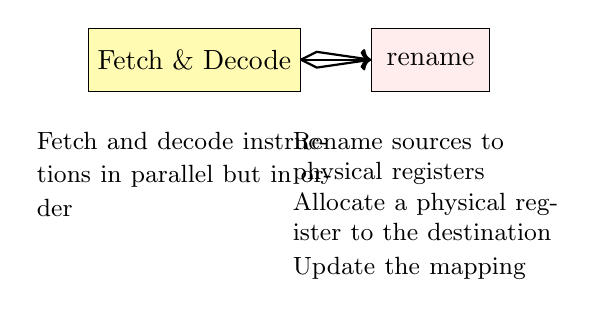
\begin{tikzpicture}[scale=1,
      block/.style={rectangle, draw, fill=yellow!30, minimum width=2cm, minimum height=0.8cm},
      rename/.style={rectangle, draw, fill=pink!30, minimum width=1.5cm, minimum height=0.8cm}]
      
      \node[block] (fetch) at (0,0) {Fetch \& Decode};
      \node[rename] (rename) at (3,0) {rename};
      
      % Multiple arrows from fetch to rename
      \foreach \y in {-0.1, 0, 0.1} {
        \draw[->, thick] (fetch.east) -- ++(0.2,\y) -- (rename.west);
      }
      
      % Annotations
      \node[text width=4cm, below] at (0,-0.8) {\small Fetch and decode instructions in parallel but in order};
      \node[text width=3.5cm, below] at (3,-0.8) {\small 
        Rename sources to physical registers\\
        Allocate a physical register to the destination\\
        Update the mapping};
    \end{tikzpicture}
  \end{center}
\end{frame}

\begin{frame}{A Superscalar OOO Machine}
  \begin{center}
    \colorbox{gray!20}{\textbf{In-order}}
    
    \vspace{0.3cm}
    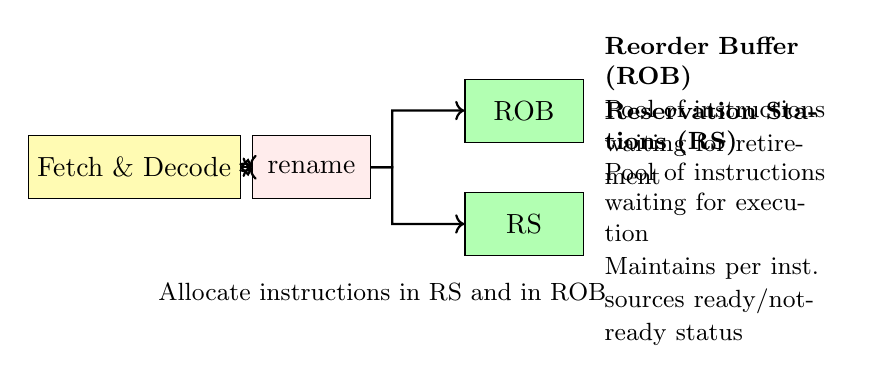
\begin{tikzpicture}[scale=0.9,
      block/.style={rectangle, draw, fill=yellow!30, minimum width=2cm, minimum height=0.8cm},
      rename/.style={rectangle, draw, fill=pink!30, minimum width=1.5cm, minimum height=0.8cm},
      pool/.style={rectangle, draw, fill=green!30, minimum width=1.5cm, minimum height=0.8cm}]
      
      \node[block] (fetch) at (0,0) {Fetch \& Decode};
      \node[rename] (rename) at (2.5,0) {rename};
      \node[pool] (rob) at (5.5,0.8) {ROB};
      \node[pool] (rs) at (5.5,-0.8) {RS};
      
      % Arrows
      \foreach \y in {-0.1, 0, 0.1} {
        \draw[->, thick] (fetch.east) -- ++(0.1,\y) -- (rename.west);
      }
      
      \draw[->, thick] (rename.east) -- ++(0.3,0) -- ++(0,0.8) -- (rob.west);
      \draw[->, thick] (rename.east) -- ++(0.3,0) -- ++(0,-0.8) -- (rs.west);
      
      % Annotations
      \node[text width=3cm, right] at (6.5,0.8) {\small \textbf{Reorder Buffer (ROB)} \\ Pool of instructions waiting for retirement};
      \node[text width=3cm, right] at (6.5,-0.8) {\small \textbf{Reservation Stations (RS)} \\ Pool of instructions waiting for execution \\ Maintains per inst. sources ready/not-ready status};
      
      \node[below] at (3.5,-1.5) {\small Allocate instructions in RS and in ROB};
    \end{tikzpicture}
  \end{center}
\end{frame}

\begin{frame}{A Superscalar OOO Machine}
  \begin{center}
    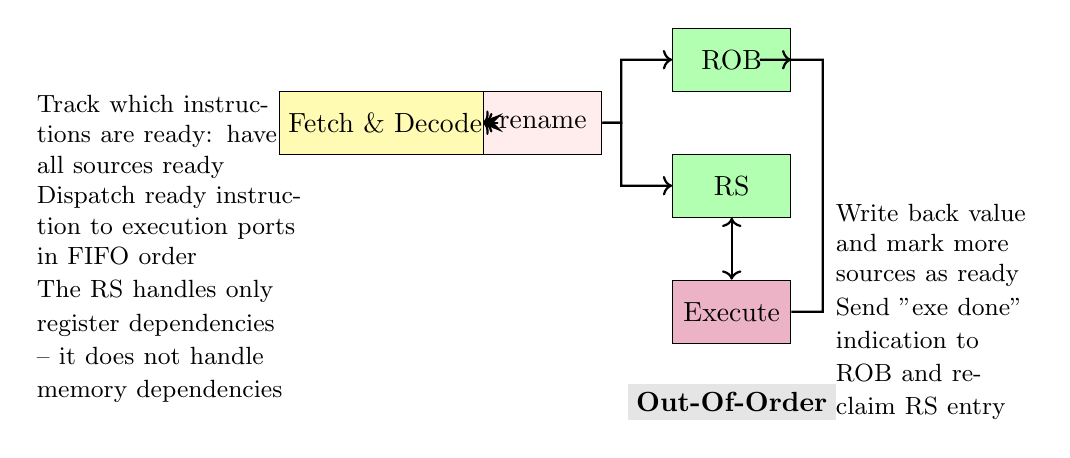
\begin{tikzpicture}[scale=0.8,
      block/.style={rectangle, draw, fill=yellow!30, minimum width=2cm, minimum height=0.8cm},
      rename/.style={rectangle, draw, fill=pink!30, minimum width=1.5cm, minimum height=0.8cm},
      pool/.style={rectangle, draw, fill=green!30, minimum width=1.5cm, minimum height=0.8cm},
      exe/.style={rectangle, draw, fill=purple!30, minimum width=1.5cm, minimum height=0.8cm}]
      
      \node[block] (fetch) at (0,0) {Fetch \& Decode};
      \node[rename] (rename) at (2.5,0) {rename};
      \node[pool] (rob) at (5.5,1) {ROB};
      \node[pool] (rs) at (5.5,-1) {RS};
      \node[exe] (execute) at (5.5,-3) {Execute};
      
      % Arrows
      \foreach \y in {-0.1, 0, 0.1} {
        \draw[->, thick] (fetch.east) -- ++(0.1,\y) -- (rename.west);
      }
      
      \draw[->, thick] (rename.east) -- ++(0.3,0) -- ++(0,1) -- (rob.west);
      \draw[->, thick] (rename.east) -- ++(0.3,0) -- ++(0,-1) -- (rs.west);
      
      % Bidirectional arrows between RS and Execute
      \draw[<->, thick] (rs.south) -- (execute.north);
      \draw[->, thick] (execute.east) -- ++(0.5,0) -- ++(0,4) -- ++(-1,0) -- (rob.east);
      
      % Annotations
      \node[text width=3.5cm, left] at (-1,-2) {\small Track which instructions are ready: have all sources ready\\
        Dispatch ready instruction to execution ports in FIFO order\\
        The RS handles only register dependencies -- it does not handle memory dependencies};
      
      \node[text width=2.5cm, right] at (7,-3) {\small Write back value and mark more sources as ready\\
        Send "exe done" indication to ROB and reclaim RS entry};
      
      \node[below] at (5.5,-4) {\colorbox{gray!20}{\textbf{Out-Of-Order}}};
    \end{tikzpicture}
  \end{center}
\end{frame}

\begin{frame}{A Superscalar OOO Machine}
  \begin{center}
    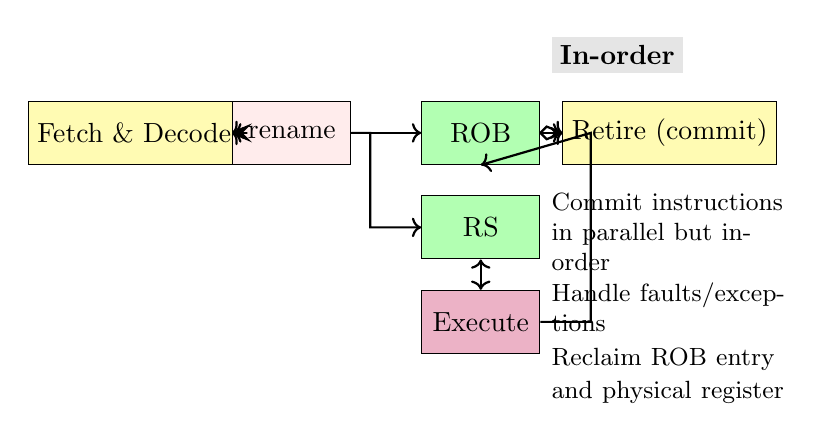
\begin{tikzpicture}[scale=0.8,
      block/.style={rectangle, draw, fill=yellow!30, minimum width=2cm, minimum height=0.8cm},
      rename/.style={rectangle, draw, fill=pink!30, minimum width=1.5cm, minimum height=0.8cm},
      pool/.style={rectangle, draw, fill=green!30, minimum width=1.5cm, minimum height=0.8cm},
      exe/.style={rectangle, draw, fill=purple!30, minimum width=1.5cm, minimum height=0.8cm},
      retire/.style={rectangle, draw, fill=yellow!30, minimum width=1.5cm, minimum height=0.8cm}]
      
      \node[block] (fetch) at (0,0) {Fetch \& Decode};
      \node[rename] (rename) at (2.5,0) {rename};
      \node[pool] (rob) at (5.5,0) {ROB};
      \node[pool] (rs) at (5.5,-1.5) {RS};
      \node[exe] (execute) at (5.5,-3) {Execute};
      \node[retire] (retire) at (8.5,0) {Retire (commit)};
      
      % Arrows
      \foreach \y in {-0.1, 0, 0.1} {
        \draw[->, thick] (fetch.east) -- ++(0.1,\y) -- (rename.west);
      }
      
      \draw[->, thick] (rename.east) -- (rob.west);
      \draw[->, thick] (rename.east) -- ++(0.3,0) -- ++(0,-1.5) -- (rs.west);
      
      % Bidirectional arrows between RS and Execute
      \draw[<->, thick] (rs.south) -- (execute.north);
      \draw[->, thick] (execute.east) -- ++(0.8,0) -- ++(0,3) -- (rob.south);
      
      % ROB to Retire
      \foreach \y in {-0.1, 0, 0.1} {
        \draw[->, thick] (rob.east) -- ++(0.1,\y) -- (retire.west);
      }
      
      % Annotations
      \node[text width=3cm, above] at (8.5,0.8) {\colorbox{gray!20}{\textbf{In-order}}};
      \node[text width=3cm, below] at (8.5,-0.8) {\small Commit instructions in parallel but in-order\\
        Handle faults/exceptions\\
        Reclaim ROB entry and physical register};
    \end{tikzpicture}
  \end{center}
\end{frame}
\end{document}